\label{sec:training}

The following section deals with the training process of YOLO and \ac{MUnet}.
For both networks similar experiments were performed each sub-experiment was repeated three times each with a different random seed.
The used seeds were: \{42, 1337, 0xDEADBEEF\}

First an initial learning rate search was performed.
Here six to seven learning rates were tested with the basic dataset.
The basic dataset is the default train / valid / test split (table \ref{tab:data_distribution} and \ref{tab:yolo_classes}) without any pre-augmentations of the training set.
The best performing learning rate was taken as the baseline for following experiments.

The second conducted experiment was a search for the optimal configuration of so called offline augmentations.
Offline augmentations are a 90\textdegree, 180\textdegree\ and a 270\textdegree\  rotation of the original image, as well as a horizontal flip and again the three rotations of the flipped image.
Furthermore, as has been described in section \ref{sec:data}, for some images a mask has been created, which is projected on different checkered background images to increase the amount of those.
This augmentation is referred to as projection or copy-paste augmentation.
The search for the optimal configuration was performed by training every possible combination of the three described offline augmentations.
Again, the best performing combination was used as the baseline for the next experiment.
Note that the flip and rotation augmentation change the class of an underlying bounding box due to the nature of the dataset, therefore augmentation complexity is increased since all labels have to be recalculated and the class has to be adapted, hence the augmentations were done before the begin of the training.

Afterwards, an ablation study was performed for various augmentations, with different parameters.
The augmentations in that study are also referred to as online augmentations, since they were performed at training time.
The occurrence probability of those augmentations was set to 50\%.
Since the augmentations slightly differ for each network they are explained in the respective subsection.

The last experiment step was formed by a fine tuning step, where a grid search was performed.
The grid search always utilized the best performing offline and online augmentations and consisted of various learning rates, batch sizes and loss functions.

Finally after training each network, a threshold fine-tuning was performed for each network and other improvement strategies were tested, such as \ac{TTA}.

%%%%%%%%%%%%%%%%%%%%%%%%%%%%%%%%%%%%%%%%%%%%%%%%%%%%%%%%%%%%%%%%%%%%%%%%%%%%%%%%%%%%%%%%
%% YOLO TRAINING
%%%%%%%%%%%%%%%%%%%%%%%%%%%%%%%%%%%%%%%%%%%%%%%%%%%%%%%%%%%%%%%%%%%%%%%%%%%%%%%%%%%%%%%%

\subsection{YOLOv4-Tiny}
\label{sec:training_yolo}

To perform any experiments with the \ac{YOLO} network, first an initial configuration was defined.
This configuration is given in table \ref{tab:initial_yolo_config}, where the default parameters of the utilized YOLO repository were used.
All networks were trained for 4000 steps (batches) and no early stopping was performed.

\begin{table}[H]
\footnotesize
\begin{center}
\begin{tabular}{|l|l|}

\hline
\textbf{Batch Size} & $64$\\
\hline
\textbf{Loss} & CIoU \\
\hline
\textbf{Optimizer} & \ac{SGD} with Momentum ($\mu = 0.9$)\\
\hline
\textbf{Burn in} & 1000 steps \\
\hline
\textbf{Input Size} & $608 \times 608 \times 1$ (gray scale) \\
\hline

\end{tabular}
\caption{The initial training configuration for the experiments performed with the YOLO network.}
\label{tab:initial_yolo_config}
\end{center}
\end{table}

Redmon et al. have pointed out that training \ac{YOLO} is unstable, when the full learning rate is applied without proper scheduling \cite{yolov2}.
This was also tested in this thesis and can be confirmed.
All learning rates which were tested in the initial learning rate search diverged when used without a scheduling mechanism.
The proposed scheduling function by Redmon et al., which is still used in the current \ac{YOLOv4} \cite{yolov4}, is given by the following formula:

\begin{equation}
    lr(step) =
    \begin{cases}
        lr_{base} * (\frac{step}{burn\_in})^4 & \textbf{if } step < burn\_in\\
        lr_{base}                             & \textbf{else}
    \end{cases}
\end{equation}

All trained experiments were optimized for a slightly changed COCO mAP metric.
COCO uses a $mAP0.5:0.95:0.05$, while in this thesis $mAP0.5:0.75:0.05$ is used, since an \ac{IoU} of $0.75$ is considered to be enough for the whole system to work properly in most circumstances.
All experiments are optimized for this metric, which means that at every step the mAP is calculated for the whole validation set and if the mAP is better than the previously calculated mAP, the weights of the network are stored and used for further evaluation.

\subsubsection{Experiment: Initial Learning Rate Search}

The first experiment was executed to find an initial learning rate.
The parameters for the network were set to the ones in table \ref{tab:initial_yolo_config} and kept for all training runs.
The results of the training runs can be found in figure \ref{fig:yolo_lr_experiment_results}, where the mean of mAP for the three performed runs is shown for each learning rate.
The full results of the learning rate search with classwise performance can be found in table \ref{tab:yolo_init_lr_results}.
It can be observed that the learning rate $0.001$ has the highest \ac{mAP}, therefore it is selected as the default learning rate for further experiments.
In this experiment the text class and especially the arrow classes showed consistently bad performance over all learning rates.

\begin{figure}
\begin{center}
    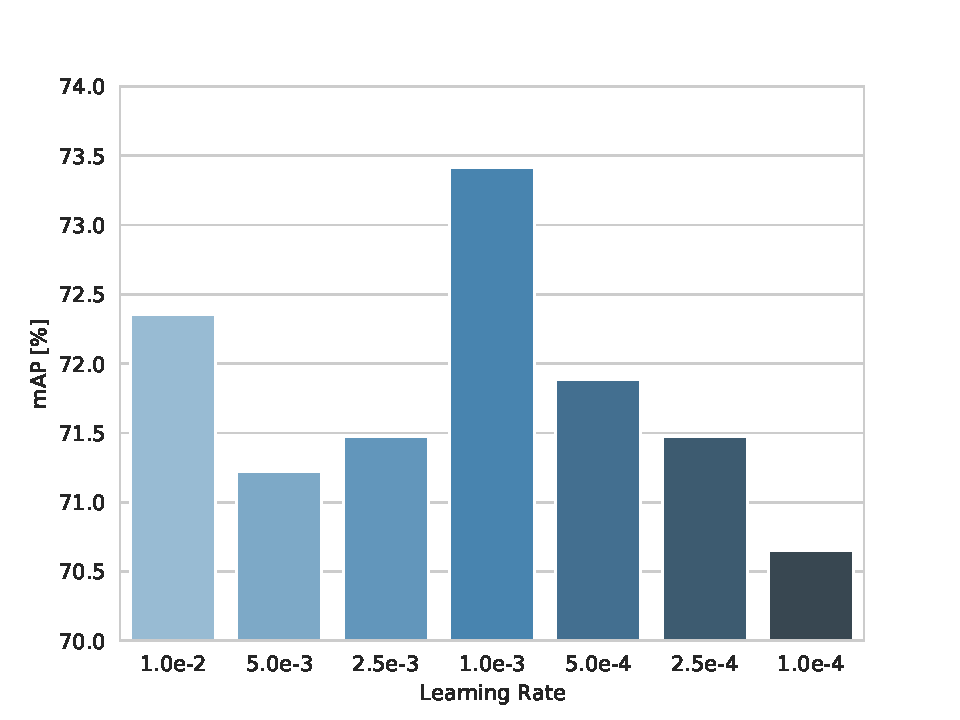
\includegraphics[width=13cm]{imgs/yolo_lr_experiment.pdf}
    \caption{The results of the initial learning rate search shown on the validation set, as the mean of the mAPs of three separate training runs.}
    \label{fig:yolo_lr_experiment_results}
\end{center}
\end{figure}


\subsubsection{Experiment: Offline Augmentations}

This experiment was conducted to find the optimal configuration of offline augmentations, where the offline augmentations are projection (copy-paste augmentation \cite{copypaste_aug}), three 90\textdegree\ rotations and a horizontal flip.
If both the rotation and the flip augmentation are selected at the same time, then additionally the flipped image is rotated three times.
Again for all runs the YOLO configuration from the previous experiment was used, but additionally now the learning rate is set to the best performing one from the learning rate search experiment, which is: $lr = 0.001$.

% \begin{table}[H]
% \footnotesize
% \begin{center}
% \begin{tabular}{|l|l|}

% \hline
% \textbf{Learning Rate} & $1e^{-3}$ \\
% \hline
% \textbf{Batch Size} & $64$\\
% \hline
% \textbf{Loss} & CIoU \\
% \hline
% \textbf{Optimizer} & SGD with Momentum ($\mu = 0.9$)\\
% \hline
% \textbf{Burn in} & 1000 steps \\
% \hline
% \textbf{Dataset} & Pre-augmented with respective experiment configuration \\
% \hline

% \end{tabular}
% \caption{The training configuration for the offline augmentation experiment, where the learning rate is set to the best performing learning rate from the learning rate search and the data is pre-augmented with the respective experiment configuration.}
% \label{tab:yolo_offline_aug_config}
% \end{center}
% \end{table}

\begin{figure}
\begin{center}
    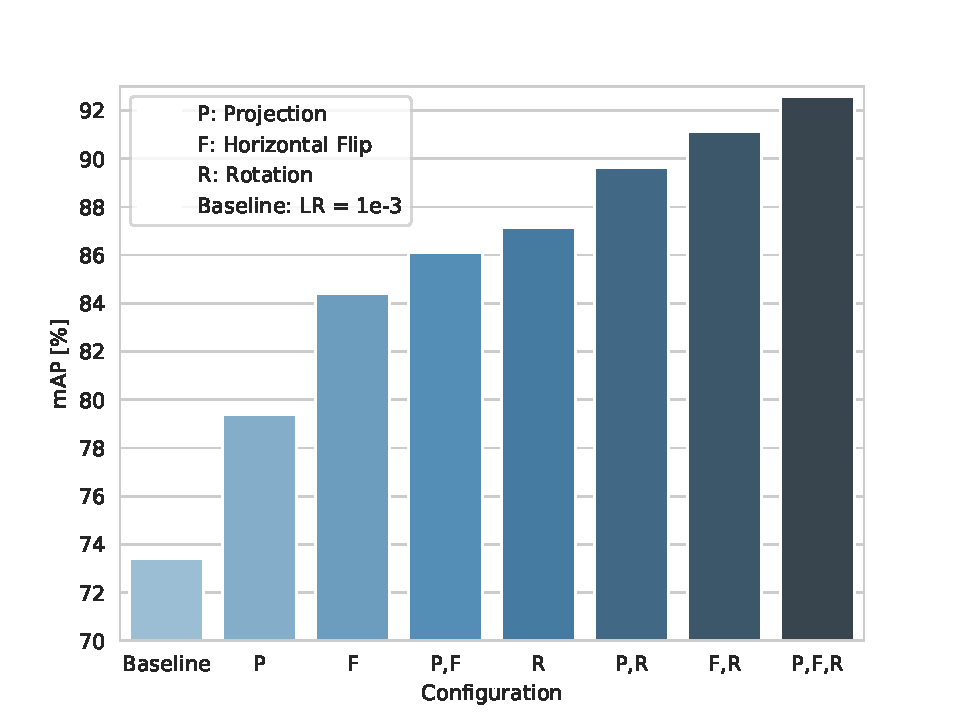
\includegraphics[width=13cm]{imgs/yolo_offline_aug_experiment.pdf}
    \caption{The results of the offline augmentation with the different offline augmentation configurations compared with the results of the best performing learning rate (baseline). When rotation and flip are enabled simultaneously the flipped image also gets rotated three times by 90\textdegree. Results are given as the mean of the mAP of three separate training runs.}
    \label{fig:yolo_offline_aug_results}
\end{center}
\end{figure}

The full results with classwise \ac{AP} can be found in table \ref{tab:yolo_offline_aug_results}.
The results for this experiment are also shown in figure \ref{fig:yolo_offline_aug_results}, where a clear trend emerges.
When looking at the results as an ablation it can be seen that each offline augmentation brought an increase in \ac{mAP} and the combination of those too.
Rotation has an absolute increase in mAP, when compared to the baseline (the best performing learning rate), of $13.725\%$, flip shows an increase of $11.000\%$ and the copy-paste augmentation shows an increase of $5.988\%$.
The best configuration is, as expected, the one where all three augmentations are used simultaneously and it has an increase in \ac{mAP} of $19.163\%$.
When comparing the classwise results of the best performing configuration with the classwise results of the baseline, it can be observed that all \ac{ECC} classes have reached a \ac{mAP} greater than $90\%$.
The text and arrow classes have also greatly increased.
Text shows an increase of $24.485\%$ and the mean over the arrow classes shows an increase of $47.988\%$, however those two classes are still not near the desired performance observed at the \acp{ECC}.
It should be pointed out that especially the increase in the text class is very interesting, because this is the only class which is not rotation and flip invariant, i.e. flipping a diode produces again a diode for human perception, just with a different orientation.
However flipping a text will produce something no more really interpretable for the human perception.
An explanation why there is still an increase in recognition performance could be that the network starts learning blob like regions, which are located near \acp{ECC}, instead of specific features related to the different textual annotations.


\subsubsection{Experiment: Online Augmentations}

The next presented experiment was an ablation study performed on the following augmentations:
\begin{itemize}
    \item Rotation: 10\textdegree, 20\textdegree, 30\textdegree\ (maximum angle to rotate the base image +- value)
    \item Scale: 10\%, 20\%, 30\% (the maximum percentage of the base scale to change +- value)
    \item SafeCrop: 70\%, 80\%, 90\% (the maximum size of the crop relative to the input image size, but considers bounding boxes such that bounding boxes are never cropped)
    \item ColorJitter: 10\%, 20\%, 30\% (the maximum percentage to change the brightness, contrast, saturation or the hue of the input image)
\end{itemize}
These augmentations are performed at runtime and are therefore also referred to as  online augmentations.
Each augmentation was applied with a probability of 50\%.
% The general configuration for this experiment is shown in table \ref{tab:yolo_online_config}
The configuration of this experiment now additionally utilizes the best combination of offline augmentations from the previous experiment.

% \begin{table}[H]
% \footnotesize
% \begin{center}
% \begin{tabular}{|l|l|}

% \hline
% \textbf{Batch Size} & $64$\\
% \hline
% \textbf{Loss} & CIoU \\
% \hline
% \textbf{Optimizer} & SGD with Momentum ($\mu = 0.9$)\\
% \hline
% \textbf{Burn in} & 1000 steps \\
% \hline
% \textbf{Dataset} & Pre-augmented with projection, flip and rotation \\
% \hline

% \end{tabular}
% \caption{The YOLO training configuration for the online augmentation experiment. The dataset is now additionally pre-augmented with the projection, flip and rotation augmentation.}
% \label{tab:yolo_online_config}
% \end{center}
% \end{table}

The detailed results can be found in the tables \ref{tab:yolo_rotation_augmentation_result}, \ref{tab:yolo_random_scale_augmentation_result}, \ref{tab:yolo_bbox_safe_crop_augmentation_result}, \ref{tab:yolo_color_jitter_augmentation_result}, for each used augmentation separately.
Further, the combined results can be found in figure \ref{fig:yolo_online_aug_results}.
The figure shows, for each augmentation and for all parameters a clear increase in \ac{mAP}.
The best performing parameters are selected to be used in the following grid search experiment.

\begin{figure}
\begin{center}
    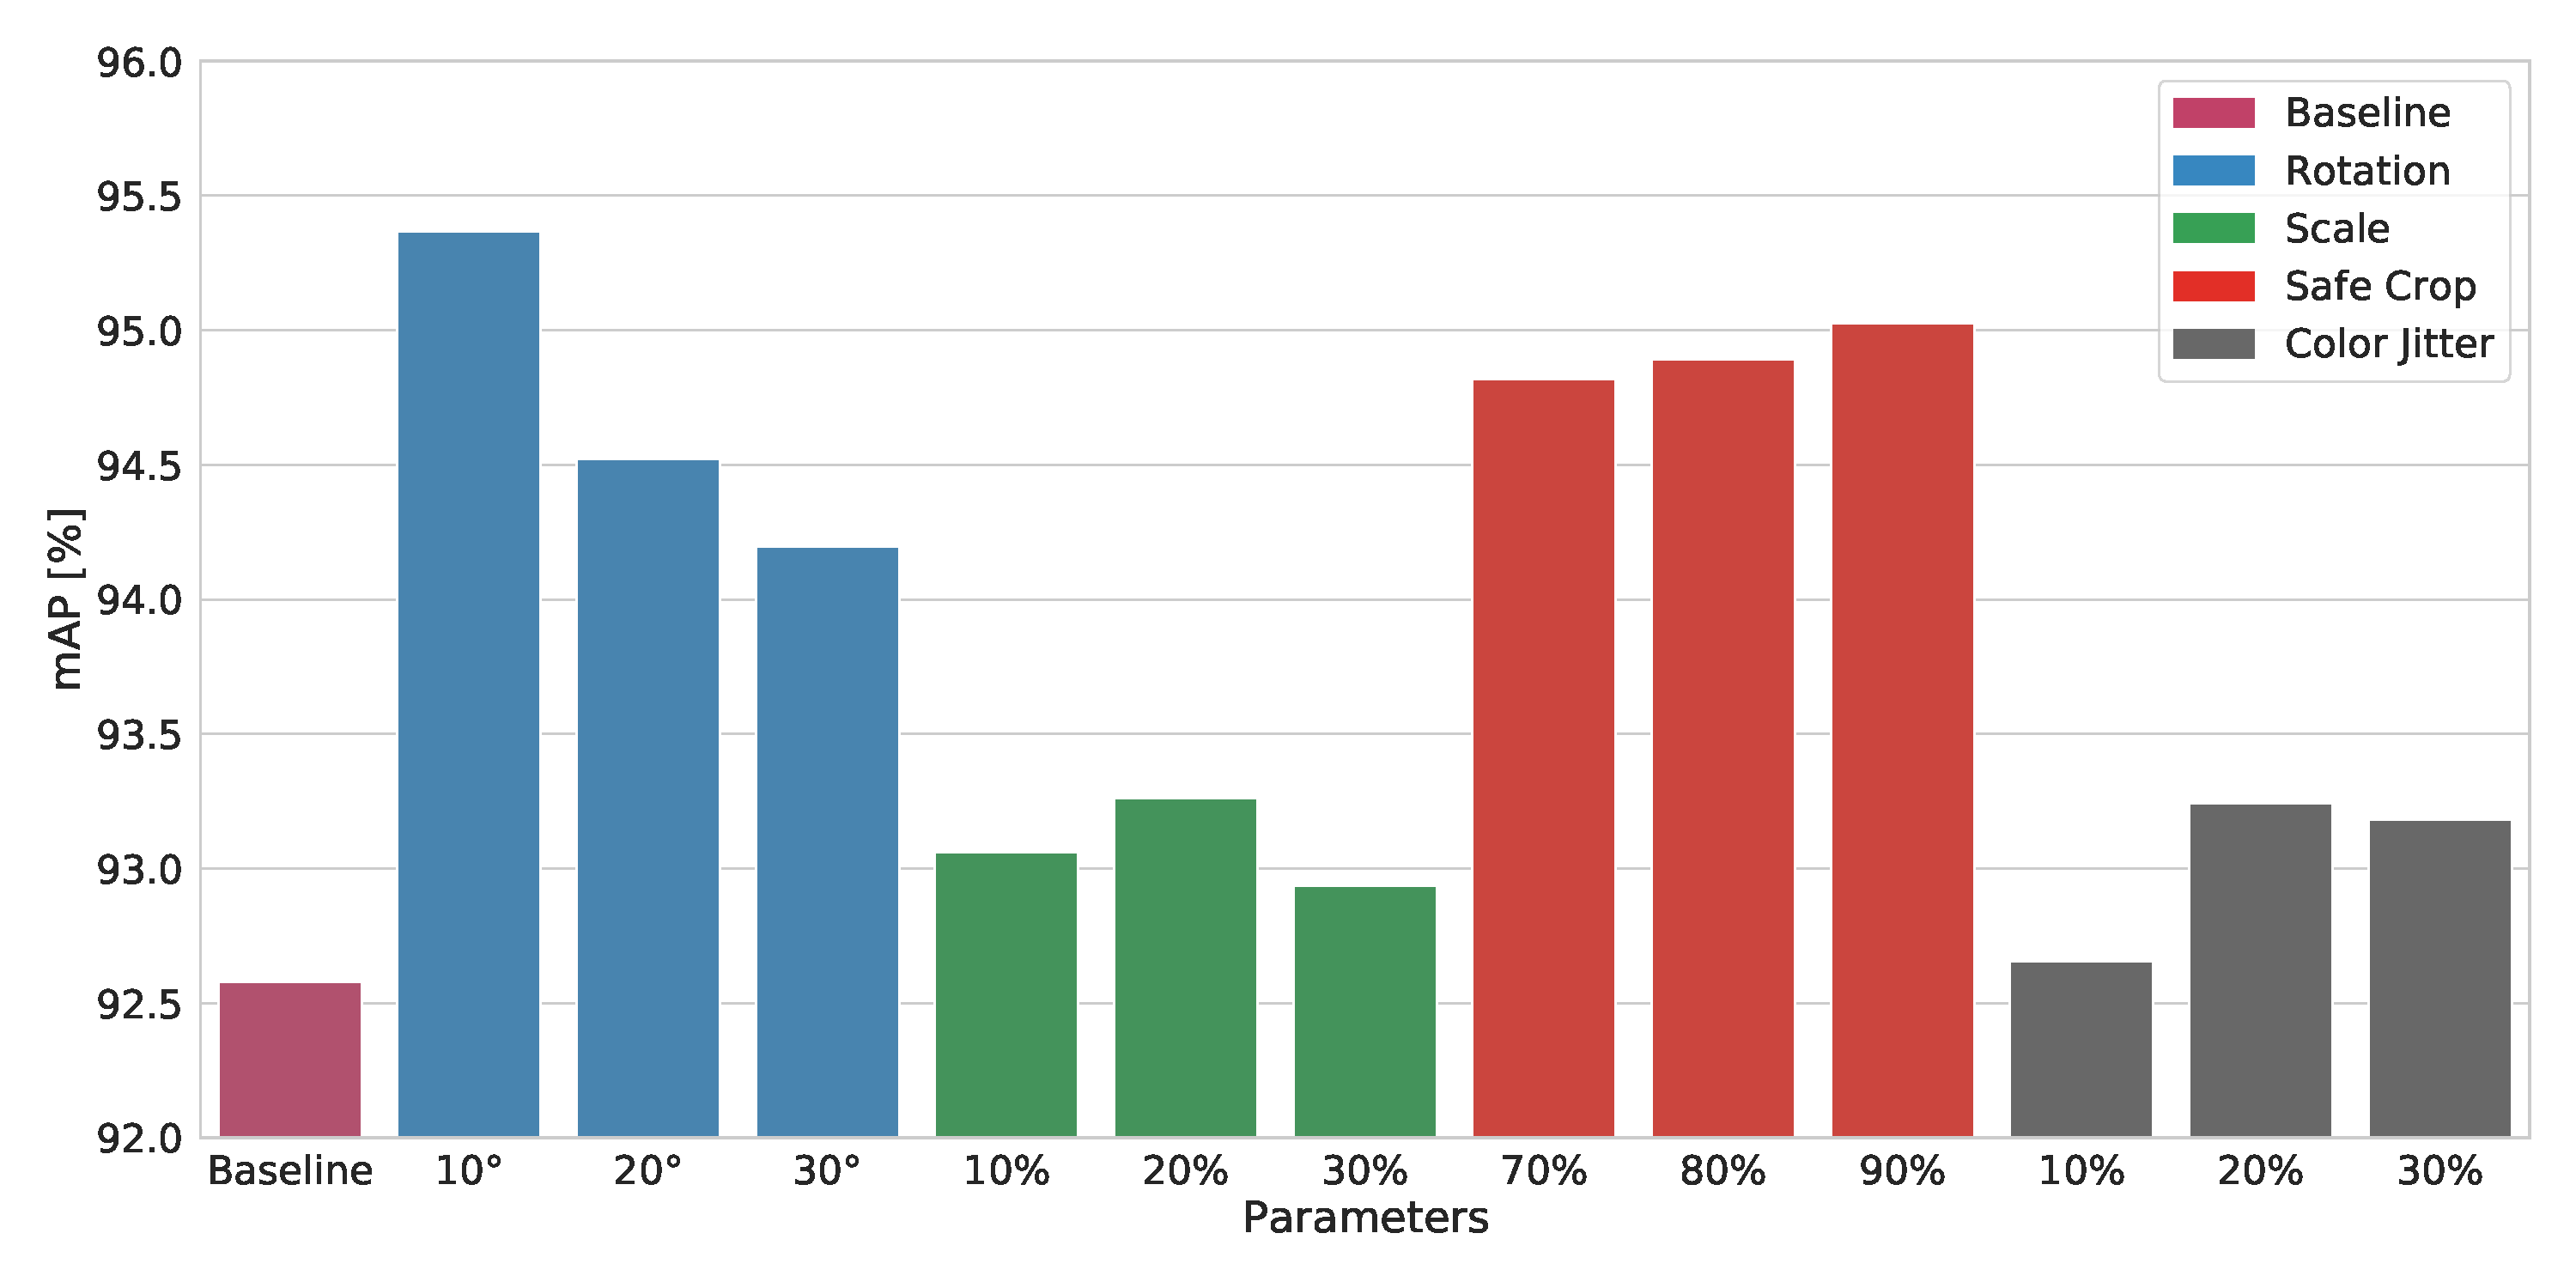
\includegraphics[width=16cm]{imgs/yolo_online_aug_experiment.pdf}
    \caption{Results of the online augmentation experiment compared to the baseline which was established in the offline augmentation experiment. Each augmentation shows a clear increase in mAP in comparison to the baseline.}
    \label{fig:yolo_online_aug_results}
\end{center}
\end{figure}

\subsubsection{Experiment: Grid Search}

The last training experiment is a grid search for finding the best learning rate, batch size and most suitable loss function.
The used parameters in the grid search are listed in table \ref{tab:yolo_grid_search_config}, seven learning rates, two batch sizes and three different types of loss functions were used.
\ac{CIoU} is also the default loss used throughout the previous experiments, while \ac{EIoU} and Focal-\ac{EIoU} are newly added for this experiment.
The $\gamma$ parameter in Focal-\ac{EIoU} was not set arbitrary, but was selected based on the experiments of the authors of \ac{EIoU} \cite{eiou}, where that $\gamma$ has shown the best results.

\begin{table}[H]
\footnotesize
\begin{center}
\begin{tabular}{|l|l|}

\hline
\textbf{Learning Rates} & $1.0e^{-2}, 5.0e^{-3}, 2.5e^{-3}, 1.0e^{-3}, 5.0e^{-4}, 2.5e^{-4}, 1.0e^{-4}$ \\
\hline
\textbf{Batch Sizes} & $32, 64$\\
\hline
\textbf{Losses} & CIoU, EIoU, Focal-EIoU ($\gamma = 0.5$) \\
\hline
\textbf{Offline Augmentations} & projection, flip, rotation \\
\hline
\textbf{Online Augmentations} & rotation = 10\textdegree, scale = 20\%, safe crop = 90\%, color jitter = 20\% \\
\hline

\end{tabular}
\caption{Configuration of the YOLO grid search experiment. The networks were trained for all possible configurations of learning rate, batch size and loss function.}
\label{tab:yolo_grid_search_config}
\end{center}
\end{table}

The full results of the grid search can be found in appendix in the tables TODO REF TABLES.
In figure \ref{fig:yolo_grid_bs_compare_results} first the batch sizes are compared.
It can be clearly seen that a batch size of 32 performed consistently worse than a batch size of 64 independently of the underlying learning rate - loss combination.
Therefore, the following evaluation of the results is only done on the networks, which were trained with a batch size of 64.

\begin{figure}
\begin{center}
    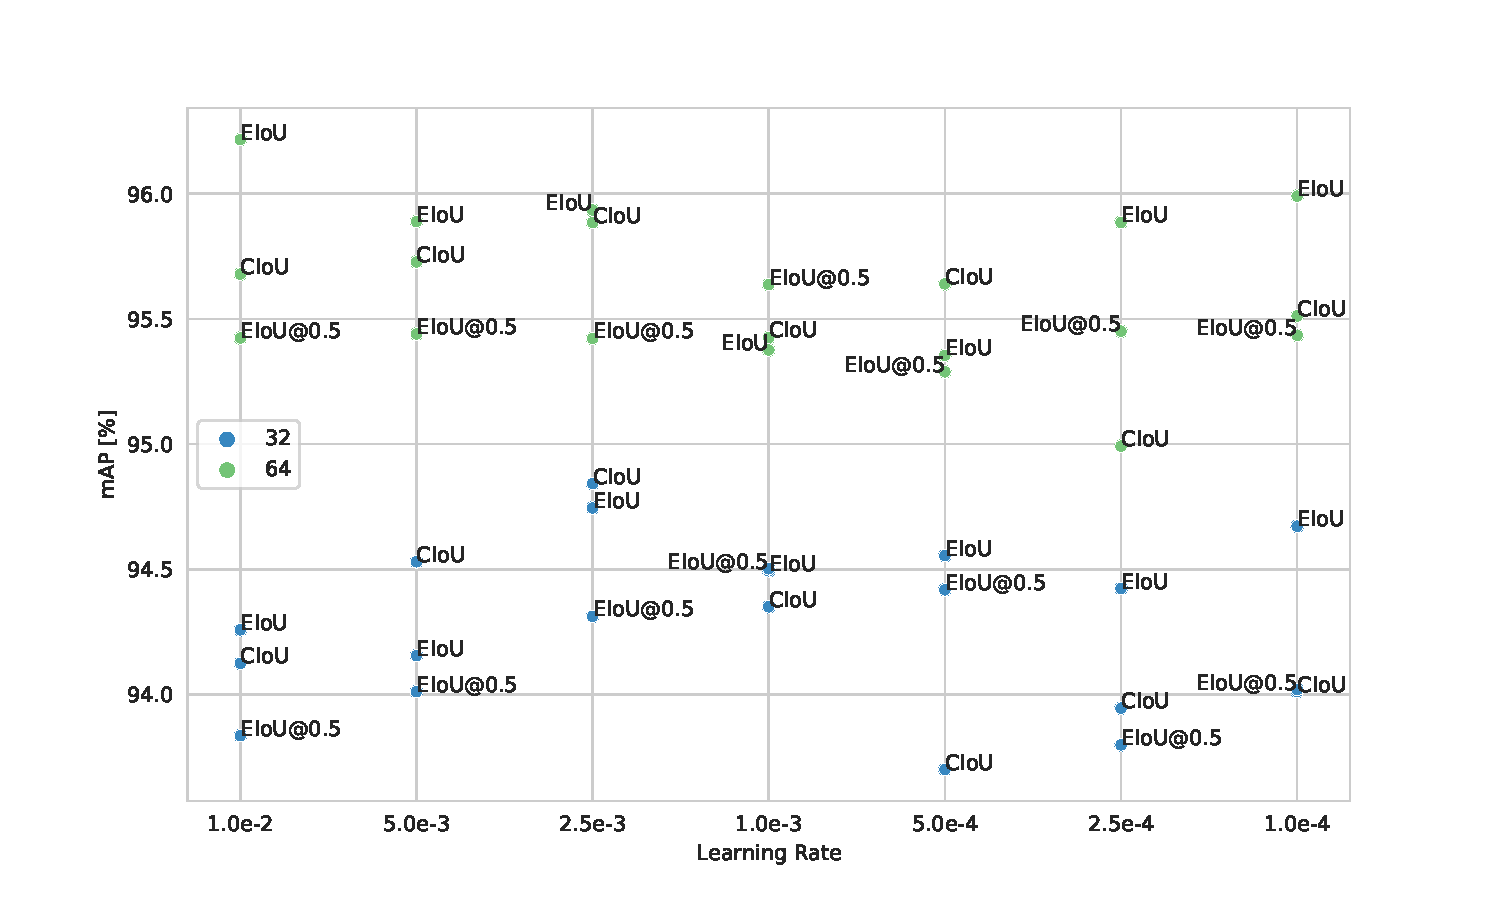
\includegraphics[width=12cm]{imgs/yolo_grid_bs_compare.pdf}
    \caption{Results of the grid search shown for all loss functions, learning rates and batch sizes.}
    \label{fig:yolo_grid_bs_compare_results}
\end{center}
\end{figure}

Figure \ref{fig:yolo_grid_heat_results} shows a heat map for all possible configurations trained with a batch size of 64.
It can be observed that networks trained with \ac{EIoU} performed better over all learning rates, while those trained with \ac{CIoU} performed second best and networks trained with Focal-\ac{EIoU} performed the worst.

\begin{figure}
\begin{center}
    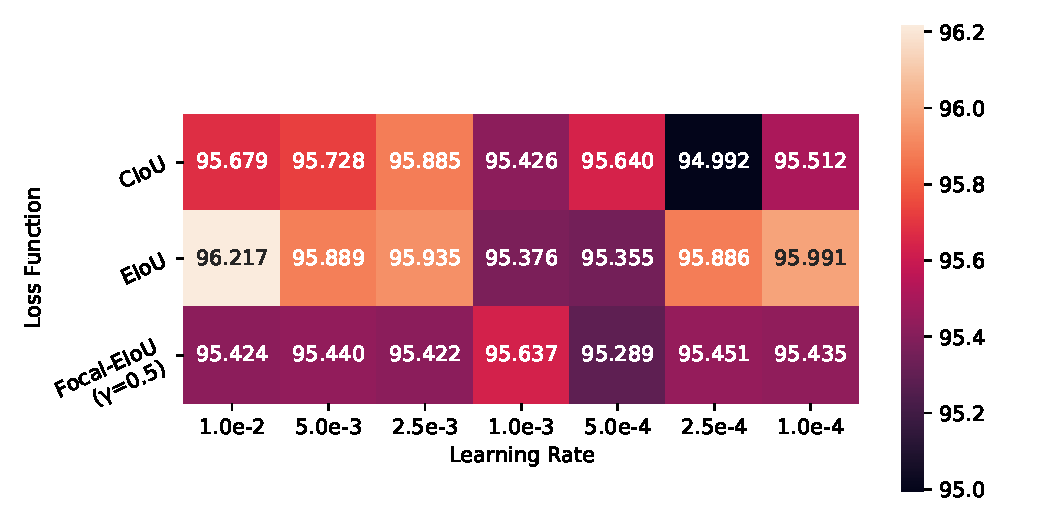
\includegraphics[width=16cm]{imgs/yolo_grid_heat.pdf}
    \caption{Results of the YOLO grid search for all used loss functions and learning rates shown for batch size 64.}
    \label{fig:yolo_grid_heat_results}
\end{center}
\end{figure}

\subsubsection{Tuning: Input Size}

Redmon et al. \cite{yolov2} trained their YOLO networks (v2, v3) with a small input resolution and after training increased it to get a further boost in performance.
Same is done in this thesis.
The networks in this thesis were trained with an input size of $608 \times 608$, which is the default input size for \ac{YOLOv4}-Tiny.
This is now tuned, by testing increasing input sizes on the validation set and selecting the best performing one.
The results of this tuning can be found in figure \ref{fig:yolo_input_size}.
The input size $736 \times 736$, shows a maximum increase in performance and is hence selected for further tuning experiments.

\begin{figure}
\begin{center}
    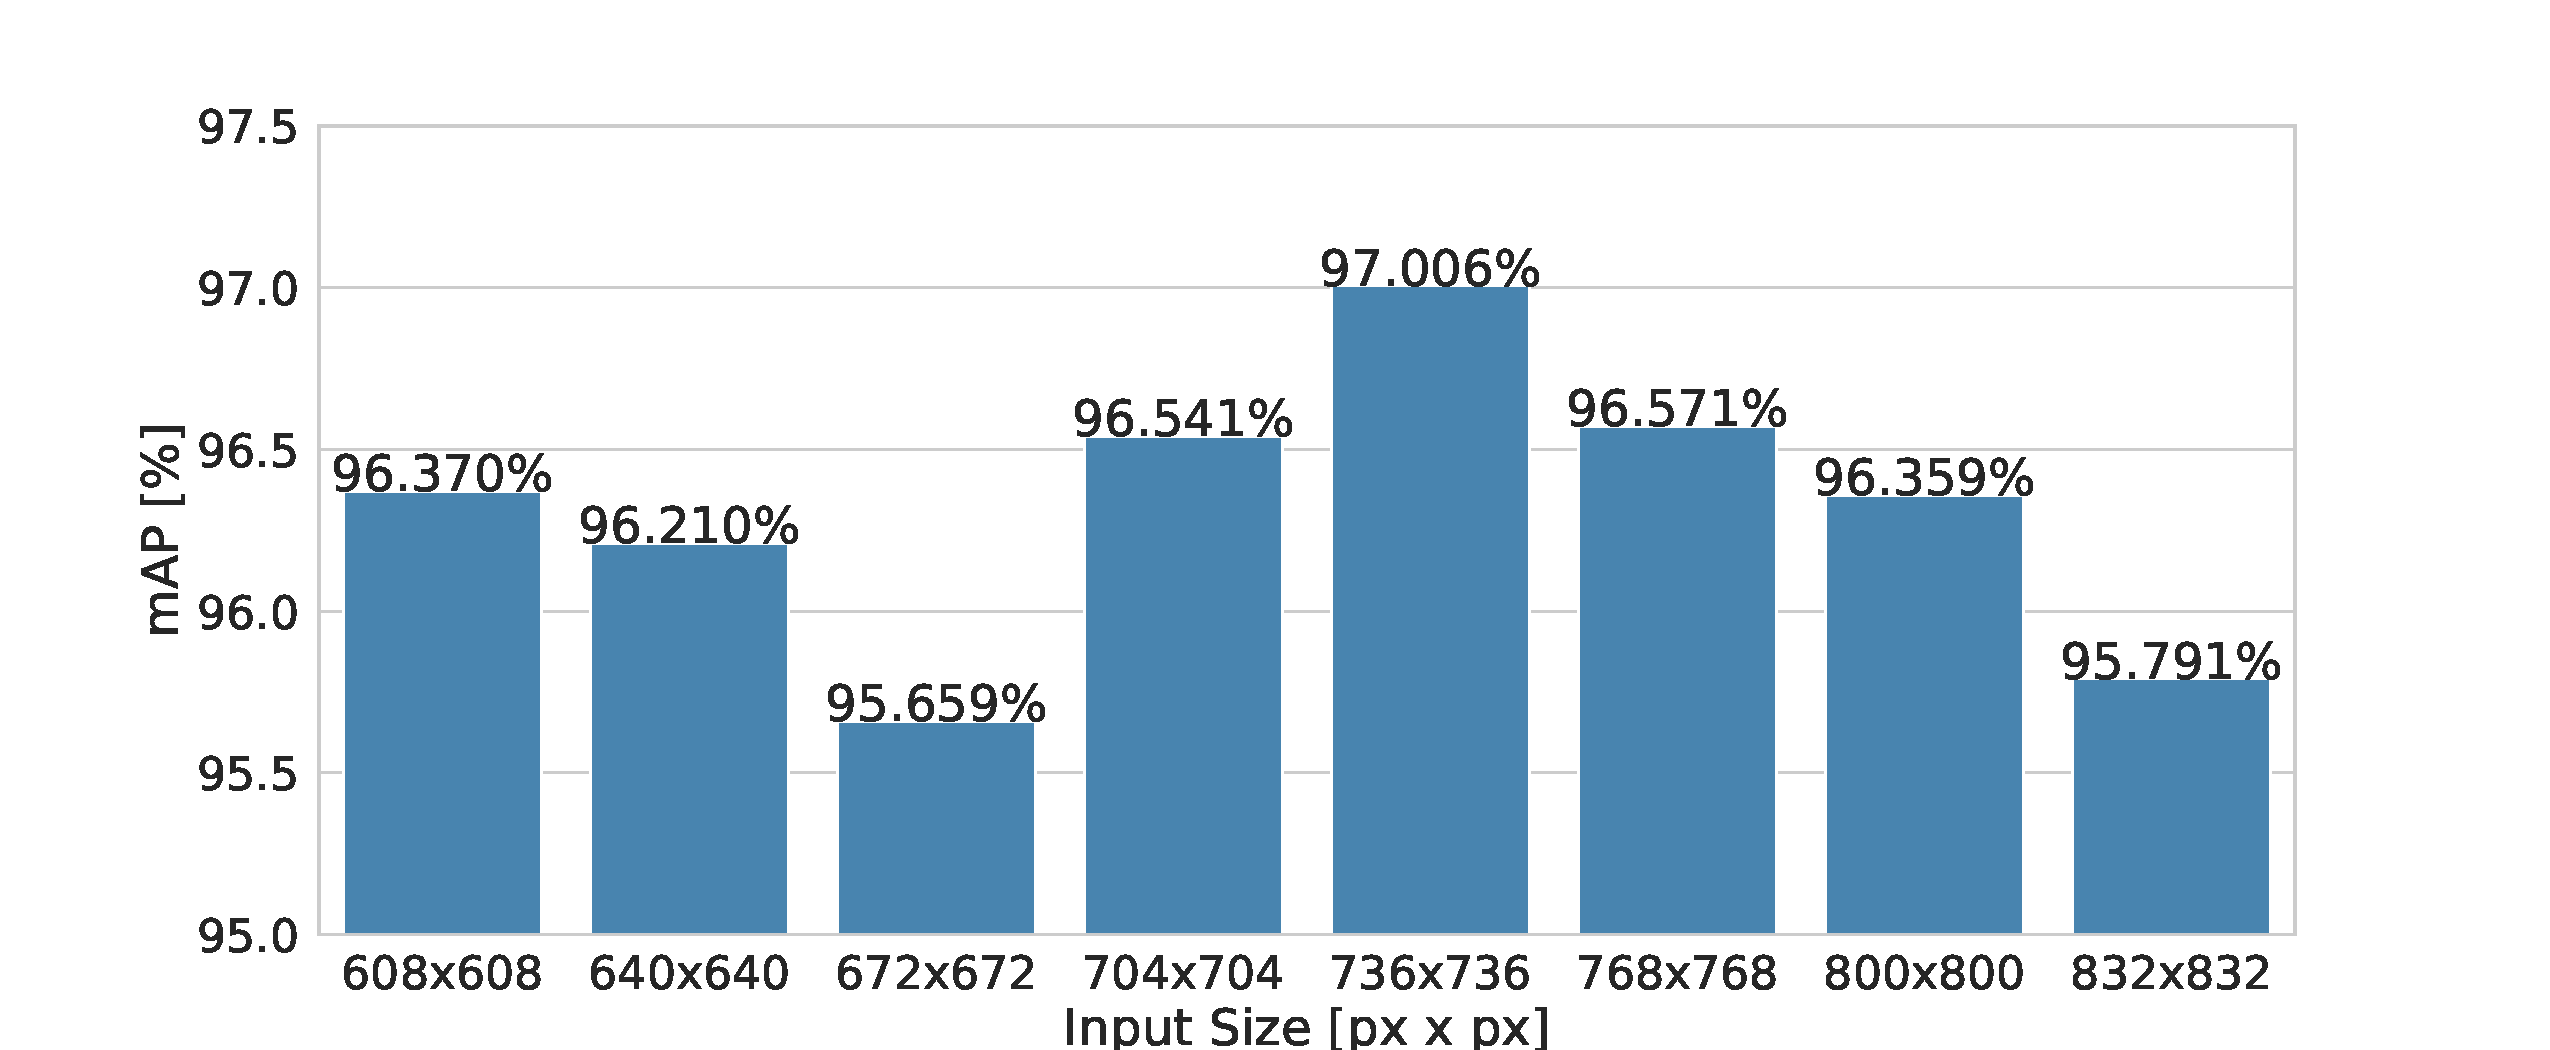
\includegraphics[width=14cm]{imgs/yolo_input_size_tuning.pdf}
    \caption{Different input sizes tested after training on the validation set.}
    \label{fig:yolo_input_size}
\end{center}
\end{figure}

\subsubsection{Tuning: Non-Maximum Suppression and Test-Time Augmentation}

YOLO predicts multiple bounding boxes per object.
To suppress unnecessary ones and keep only the most suitable, \ac{NMS} is used.
The used \ac{NMS} algorithm during all previous experiments was \ac{DIoU}-\ac{NMS} \cite{diou}.
In this subsection the results are also evaluated using the \ac{WBF} algorithm \cite{weighted_bbox_fusion}, which has shown to perform well in combination with \ac{TTA}.
Both algorithms were explained in section \ref{sec:yolo}.
All tunings are performed only on the validation dataset, with the new input size of $736 \times 736$.

First a tuning of the \ac{DIoU}-\ac{NMS} thresholds is performed.
To recall, \ac{DIoU}-\ac{NMS} takes as input two thresholds a score threshold, which will remove predictions with a prediction score below that one, and an \ac{IoU} threshold which is used to define whether two bounding boxes are the same one, i.e. if two bounding boxes have an $IoU > IoU_{thresh}$, then only the one with the maximum prediction score is kept and the other one is removed.
The tuning was performed on all possible combinations of score threshold and \ac{IoU} threshold, where both have the same parameter set.
The parameter set for both is ranging from 0.1 to 0.5 in 0.05 steps.
The results of the tuning can be found in figure \ref{fig:diou_nms_tuning}.
The best performing combination has a score threshold of 0.1 and a \ac{IoU} threshold of 0.45.


The second tuning is done using the above setup, except that now the thresholds are tuned for the \ac{WBF} algorithm.
The results of the tuning are shown in figure \ref{fig:wbf_nms_tuning}.
The best performing configuration has a score threshold of 0.15 and an \ac{IoU} threshold of 0.25.
Further, \ac{WBF} shows slightly better results with a relative improvement of 0.15\%.
This improvement was expected, since in the predictions with the DIoU-NMS, some \acp{FP} were found, where multiple bounding boxes were predicted for the same text object.
In \ac{WBF} such predictions are fused into one bounding box, hence the slight increase in performance.


In the last tuning additionally \ac{TTA} is added to the configuration.
The used augmentations are, as in the offline augmentation experiment, three 90\textdegree\ rotations of the original image, a horizontal flip and again three 90\textdegree\ rotations of the horizontally flipped image.
This experiment also uses \ac{WBF} to merge the predicted bounding boxes.
The full results of this tuning can be found in figure \ref{fig:wbf_tta_nms_tuning}, where the best configuration has a score threshold of 0.1 and an \ac{IoU} threshold of 0.45.
The relative improvement of \ac{WBF}-\ac{TTA}, compared to \ac{DIoU}-\ac{NMS} is 1.5\%.
For the sake of completeness it should be noted that, \ac{TTA} was also performed in combination with \ac{DIoU}-\ac{NMS}, but this actually slightly worsened the results, when comparing them to \ac{DIoU} without \ac{TTA}.


% \begin{figure}
% \begin{center}
%     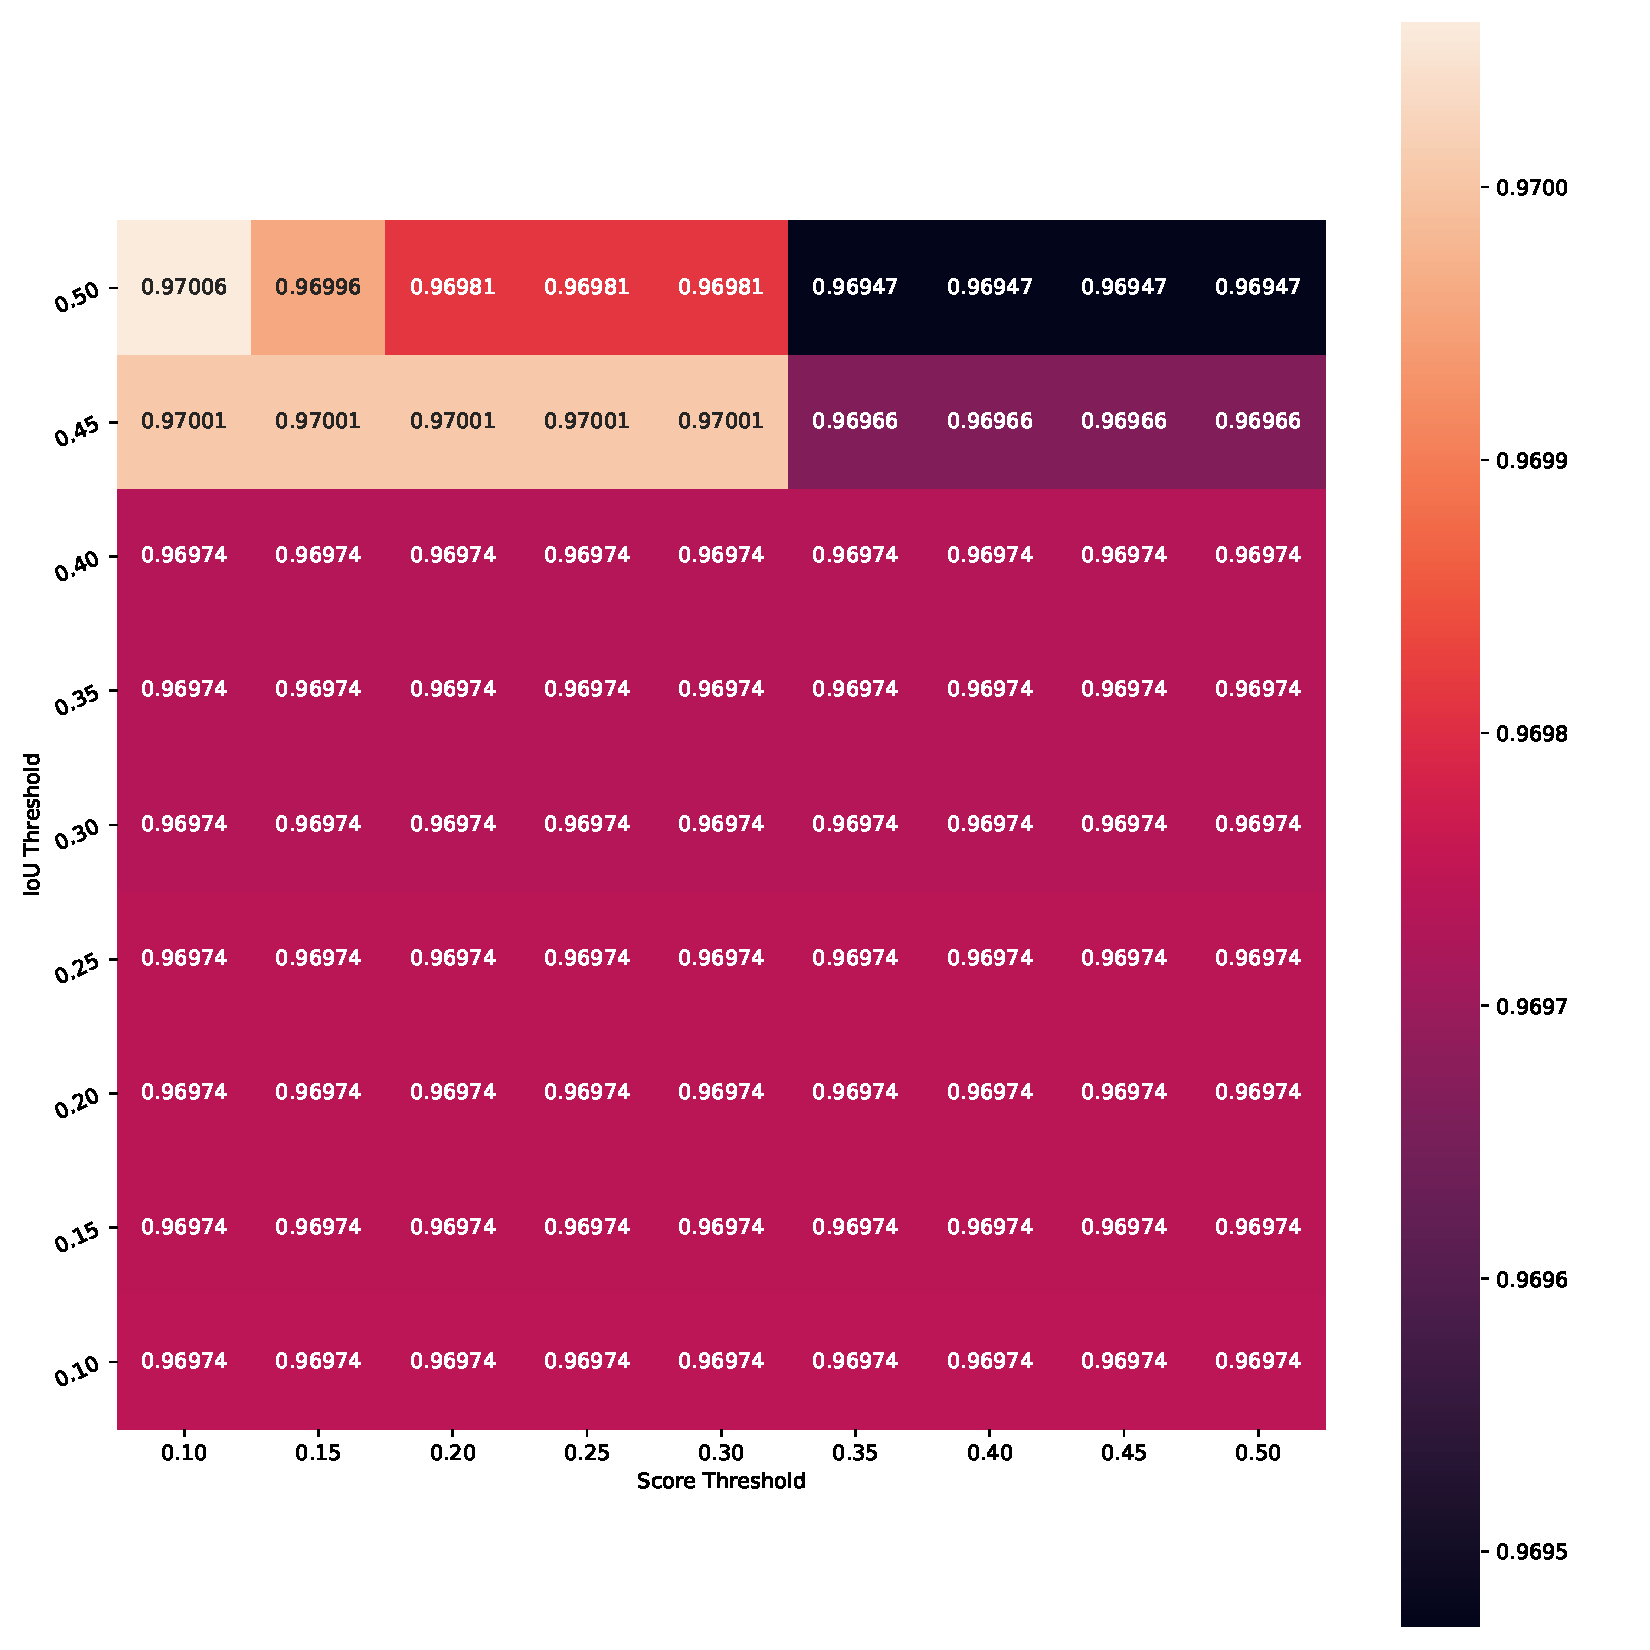
\includegraphics[width=\columnwidth]{imgs/yolo_diou_tta_heat.pdf}
%     \caption{DIOU + TTA TUNING}
%     \label{fig:diou_tta_nms_tuning}
% \end{center}
% \end{figure}

\subsubsection{Experiment: Improve Model Uncertainty Through Voting Based Thresholding in \ac{WBF}}

\ac{TTA} in combination with \ac{WBF} showed an improvement in performance, however while inspecting the predictions it was observed, that the amount of \acp{FP} has increased.
Following a predictor is defined as a model which has predicted a certain augmentation of an image.
When looking at the prediction of each predictor, it can be seen that not every predictor had predicted the same bounding box.

So to incorporate the uncertainty of each predictor the idea was to create a voting based threshold mechanism, which allows \ac{WBF} to reject bounding boxes, when the amount of casted votes on a bounding box is below a certain threshold $vote_{thresh}$.
Obviously, $vote_{thresh}$ can range from 1 to the amount of predictors.
In the case of this thesis the number of predictors is equal to the amount of images created through \ac{TTA} (8 = original image + three rotations of original + horizontal flip + three rotations of flip).
The voting was implemented directly in the repository of the \ac{WBF} algorithm.

Again, the tuning of the voting threshold was performed on every possible $voting_{thresh}$ and the obtained results are illustrated in figure \ref{fig:wbf_tta_nms_votes}.
Using a voting threshold has not shown any improvement on the validation set, hence for further evaluation a $voting_{thresh} = 1$, which is the default behavior of \ac{WBF}.

\begin{figure}[H]
\begin{center}
    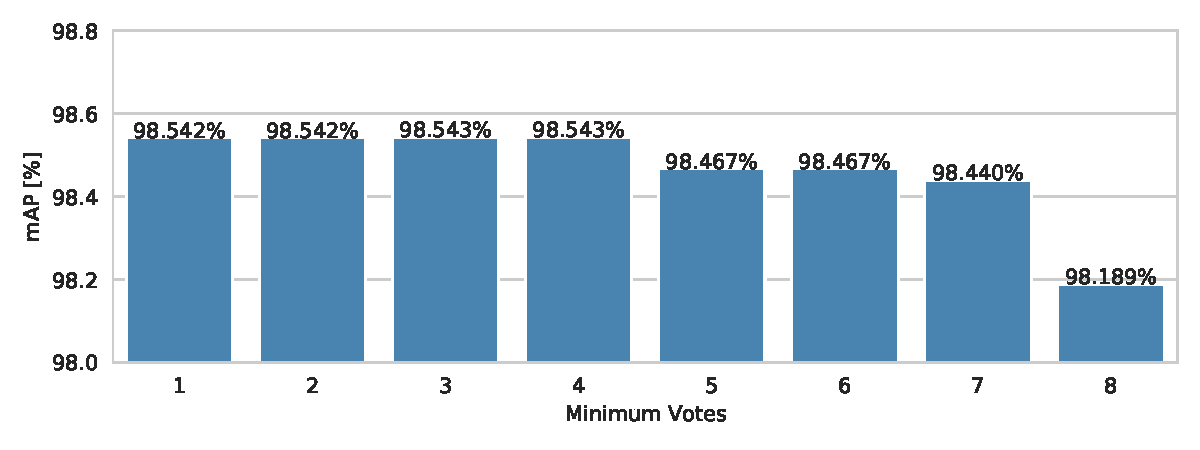
\includegraphics[width=15cm]{imgs/yolo_wbf_tta_votes.pdf}
    \caption{Results of the voting based thresholding approach to improve model performance, shown on the validation set for all possible voting thresholds.}
    \label{fig:wbf_tta_nms_votes}
\end{center}
\end{figure}

\subsubsection{Final Results}

Figure \ref{fig:yolo_tuning_combined_results} and table \ref{tab:yolo_tuning_combined_results} show the combined results of each tuning step on the validation and the test set, compared to the untuned baseline, which is the best performing network from the grid search experiment.

The first tuning A) was the tuning of the input size.
The impact of that on the validation set was way smaller than on the test set, which probably relies in the fact that the network was already tuned on the validation set during training and is hence already well optimized on that.

Then in B) and C) the two \ac{NMS} algorithms \ac{DIoU}-\ac{NMS} and \ac{WBF} were tuned.
On the validation set a slight increase can be seen for both algorithms, however on the test set that increase can only be observed for \ac{WBF}.

The last tuning in D) was additionally done using \ac{WBF} as \ac{NMS} together with \ac{TTA}.
Here, a clear increase in performance can be observed and \ac{TTA} definitely benefits the recognition performance.

Overall through tuning and \ac{TTA} a relative improvement of 2.173\% and 6.609\% could be achieved on the validation and test dataset, respectively.

\begin{figure}
\begin{center}
    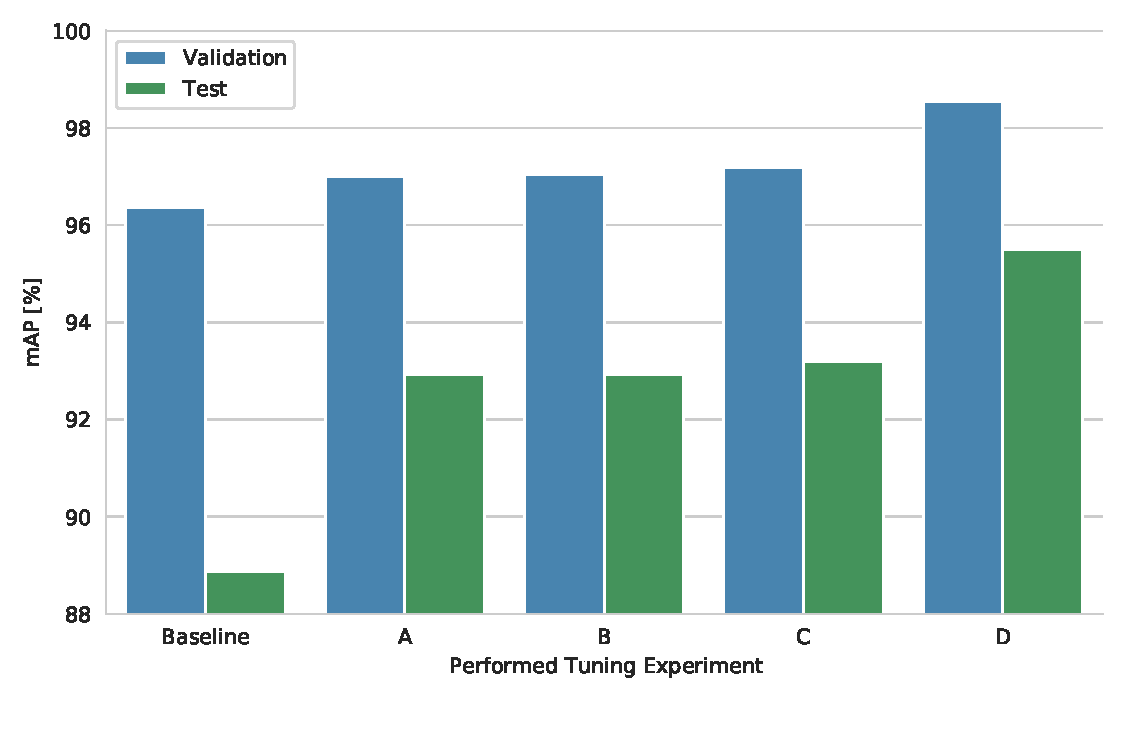
\includegraphics[width=\columnwidth]{imgs/yolo_all_tuning.pdf}
    \caption{The final results of the tuning experiment performed on the validation set, presented also with the performance on the test dataset. Specific explanation of the experiments with the optimal obtained parameters can be found in table \ref{tab:yolo_tuning_combined_results}.}
    \label{fig:yolo_tuning_combined_results}
\end{center}
\end{figure}

\begin{table}[H]
\footnotesize
\begin{center}
\begin{tabular}{|l|l|l|l|l|l|l|l|}

\hline
\textbf{Experiment in fig. \ref{fig:yolo_tuning_combined_results}} & \textbf{NMS} & \textbf{Score Thr.} & \textbf{IoU Thr.} & \textbf{Input Size} & \textbf{Val. mAP} & \textbf{Test mAP}\\
\hline
Baseline & DIoU    & 0.3  & 0.25 & $608 \times 608$ & 96.370\% & 88.883\% \\
\hline
A        & DIoU    & 0.3  & 0.25 & $736 \times 736$ & 97.006\% & 92.926\% \\
\hline
B        & DIoU    & 0.15 & 0.45 & $736 \times 736$ & 97.036\% & 92.926\% \\
\hline
C        & WBF     & 0.15 & 0.25 & $736 \times 736$ & 97.187\% & 93.188\% \\
\hline
D        & WBF-TTA & 0.1  & 0.45 & $736 \times 736$ & \cellcolor{green}98.543\% & \cellcolor{green}95.492\% \\
\hline
\end{tabular}
\caption{Results of the tuning experiment with the underlying threshold and input size combination, performed on the validation set, presented also with the performance on the test dataset. A visual representation can also be found in figure \ref{fig:yolo_tuning_combined_results}.}
\label{tab:yolo_tuning_combined_results}
\end{center}
\end{table}



%%%%%%%%%%%%%%%%%%%%%%%%%%%%%%%%%%%%%%%%%%%%%%%%%%%%%%%%%%%%%%%%%%%%%%%%%%%%%%%%%%%%%%%%
%% MUNET TRAINING
%%%%%%%%%%%%%%%%%%%%%%%%%%%%%%%%%%%%%%%%%%%%%%%%%%%%%%%%%%%%%%%%%%%%%%%%%%%%%%%%%%%%%%%%

\subsection{MobileNetV2-UNet}
\label{sec:training_munet}

In this section the training and the tuning of thresholds of the \ac{MUnet} is presented.
The experiments were conducted in the same way as with the YOLO network, as described in the beginning of this section \ref{sec:training}.
The configuration for the \ac{MUnet} is presented in table \ref{tab:munet_config}.
The selected values correspond to the initial values from the used repository.
It has been shown that transfer learning has a positive effect on the training process \cite{mobile_unet}, therefore the training of \ac{MUnet} is performed with MobileNetV2 weights, which were pretrained on the ImageNet dataset.
The backbone was pretrained on RGB images, while in this work colors are not considered to be good features.
To fit the input size of the backbone network, a grayscale image is repeated three times along the channel direction.

\begin{table}[H]
\footnotesize
\begin{center}
\begin{tabular}{|l|l|}

\hline
\textbf{Batch Sizes} & 64\\
\hline
\textbf{Loss} & Focal-EIoU ($\alpha = 0.8$, $\gamma = 2$) \\
\hline
\textbf{Optimizer} & AMSGrad ($\mu = 0.95$, $\rho = 0.999$) \\
\hline
\textbf{Input Size} & $448 \times 448 \times 3$ (gray scale image with repeated channels) \\
\hline
\textbf{Pretraining} & Backbone pretrained on ImageNet \\
\hline

\end{tabular}
\caption{Configuration of the YOLO grid search experiment. The networks were trained for all possible configurations of learning rate, batch size and loss function.}
\label{tab:munet_config}
\end{center}
\end{table}

All \ac{MUnet} training runs were executed for 7000 steps and optimized for the F1-score.
Early stopping was performed, when the F1-score metric didn't change for 3000 steps.

Further, a learning rate scheduler with the following formula was used:

\begin{equation}
    lr(step) =
    \begin{cases}
        lr_{base} / 25 & \textbf{if } \ \ \ step > 1500 \\
        lr_{base} / 5  & \textbf{elif}\ step > 1000 \\
        lr_{base}      & \textbf{else} \\
    \end{cases}
\end{equation}

\subsubsection{Experiment: Initial Learning Rate Search}

The first experiment was a search for an initial learning rate.
The results of the learning rate search can be found in figure \ref{fig:munet_lr_exp}
The learning rate 0.01 showed the best results within a reasonable standard deviation and is therefore selected as the initial learning rate for the next experiment.

\begin{figure}
\begin{center}
    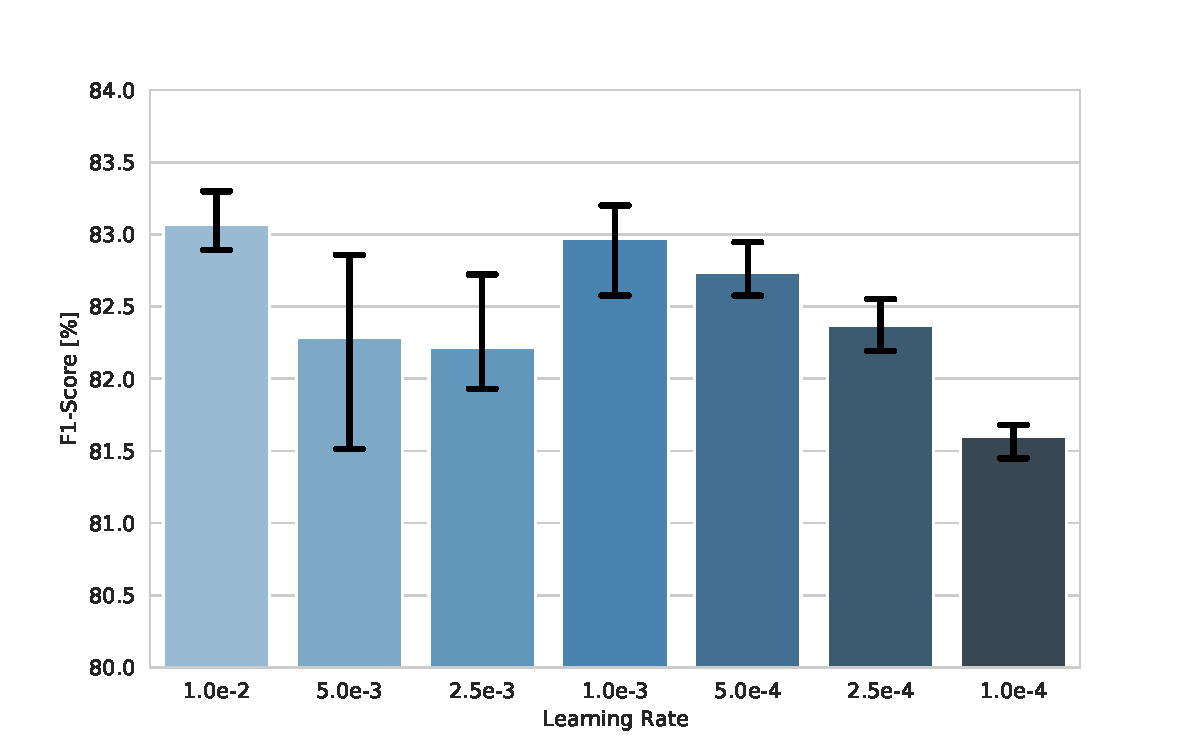
\includegraphics[width=\columnwidth]{imgs/munet_lr_exp.pdf}
    \caption{The results of the initial learning rate search shown on the validation set, as the mean F1-Score of three separate training runs.}
    \label{fig:munet_lr_exp}
\end{center}
\end{figure}

\subsubsection{Experiment: Offline Augmentations}

The next experiment was done using the learning rate from the learning rate search experiment.
The results can be found in figure \ref{fig:munet_offline_exp}.
In contrast to YOLO this experiment shows a significantly smaller increase in F1-Score in general.
Again the best performing offline augmentation combination, is the one with projection, flip and rotation.

\begin{figure}
\begin{center}
    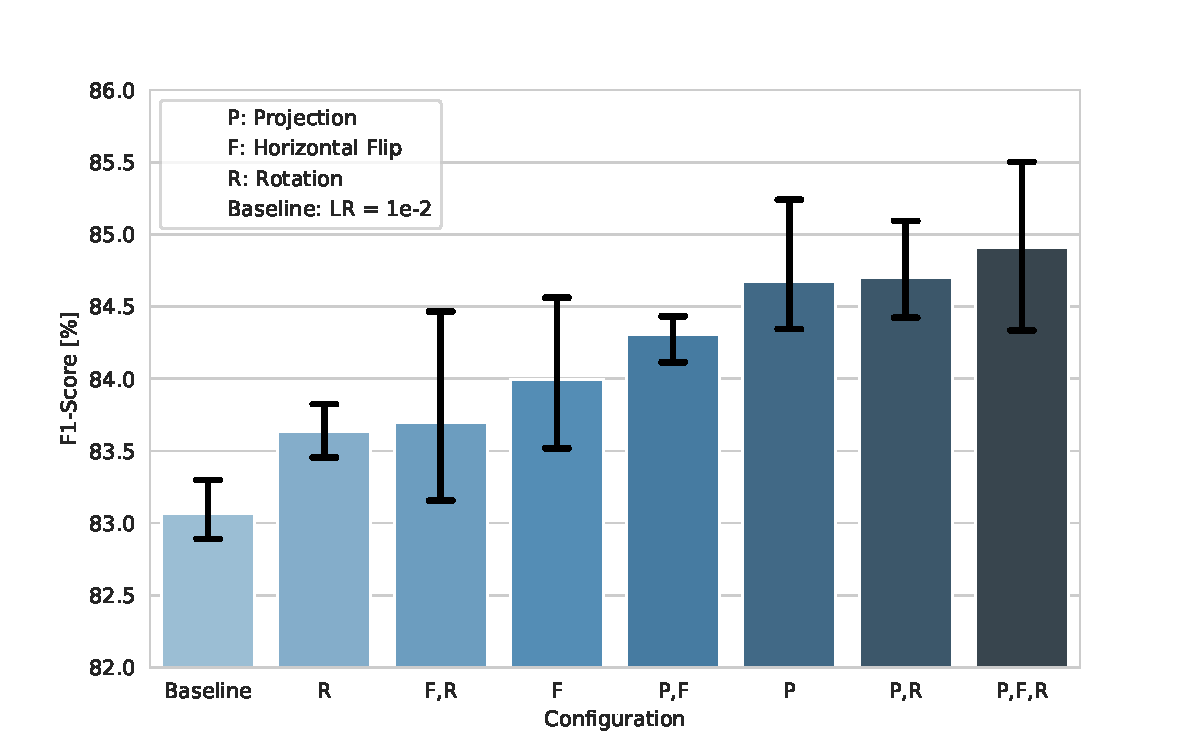
\includegraphics[width=\columnwidth]{imgs/munet_offline_aug_experiment.pdf}
    \caption{The results of the offline augmentation experiment shown on the validation set, as the mean F1-Score of three separate training runs.}
    \label{fig:munet_offline_exp}
\end{center}
\end{figure}

\subsubsection{Experiment: Online Augmentations}

The next experiment was done to find optimal parameters for the online augmentations.
Here, the same augmentations were used as in the respective YOLO experiment, except for the crop augmentation, which is now not a safe crop, but just a plain random crop, which doesn't consider the segmentation labels.
The results of this experiment can be found in figure \ref{fig:munet_online_exp}.
The only augmentation which didn't increase the performance was the scale augmentation.
It is hence not used in further experiments.
From the other augmentations again the one with the best performing parameter was selected for the following grid search.
In table \ref{tab:munet_grid_params} the selected augmentations with their respective parameters are shown.

\begin{figure}
\begin{center}
    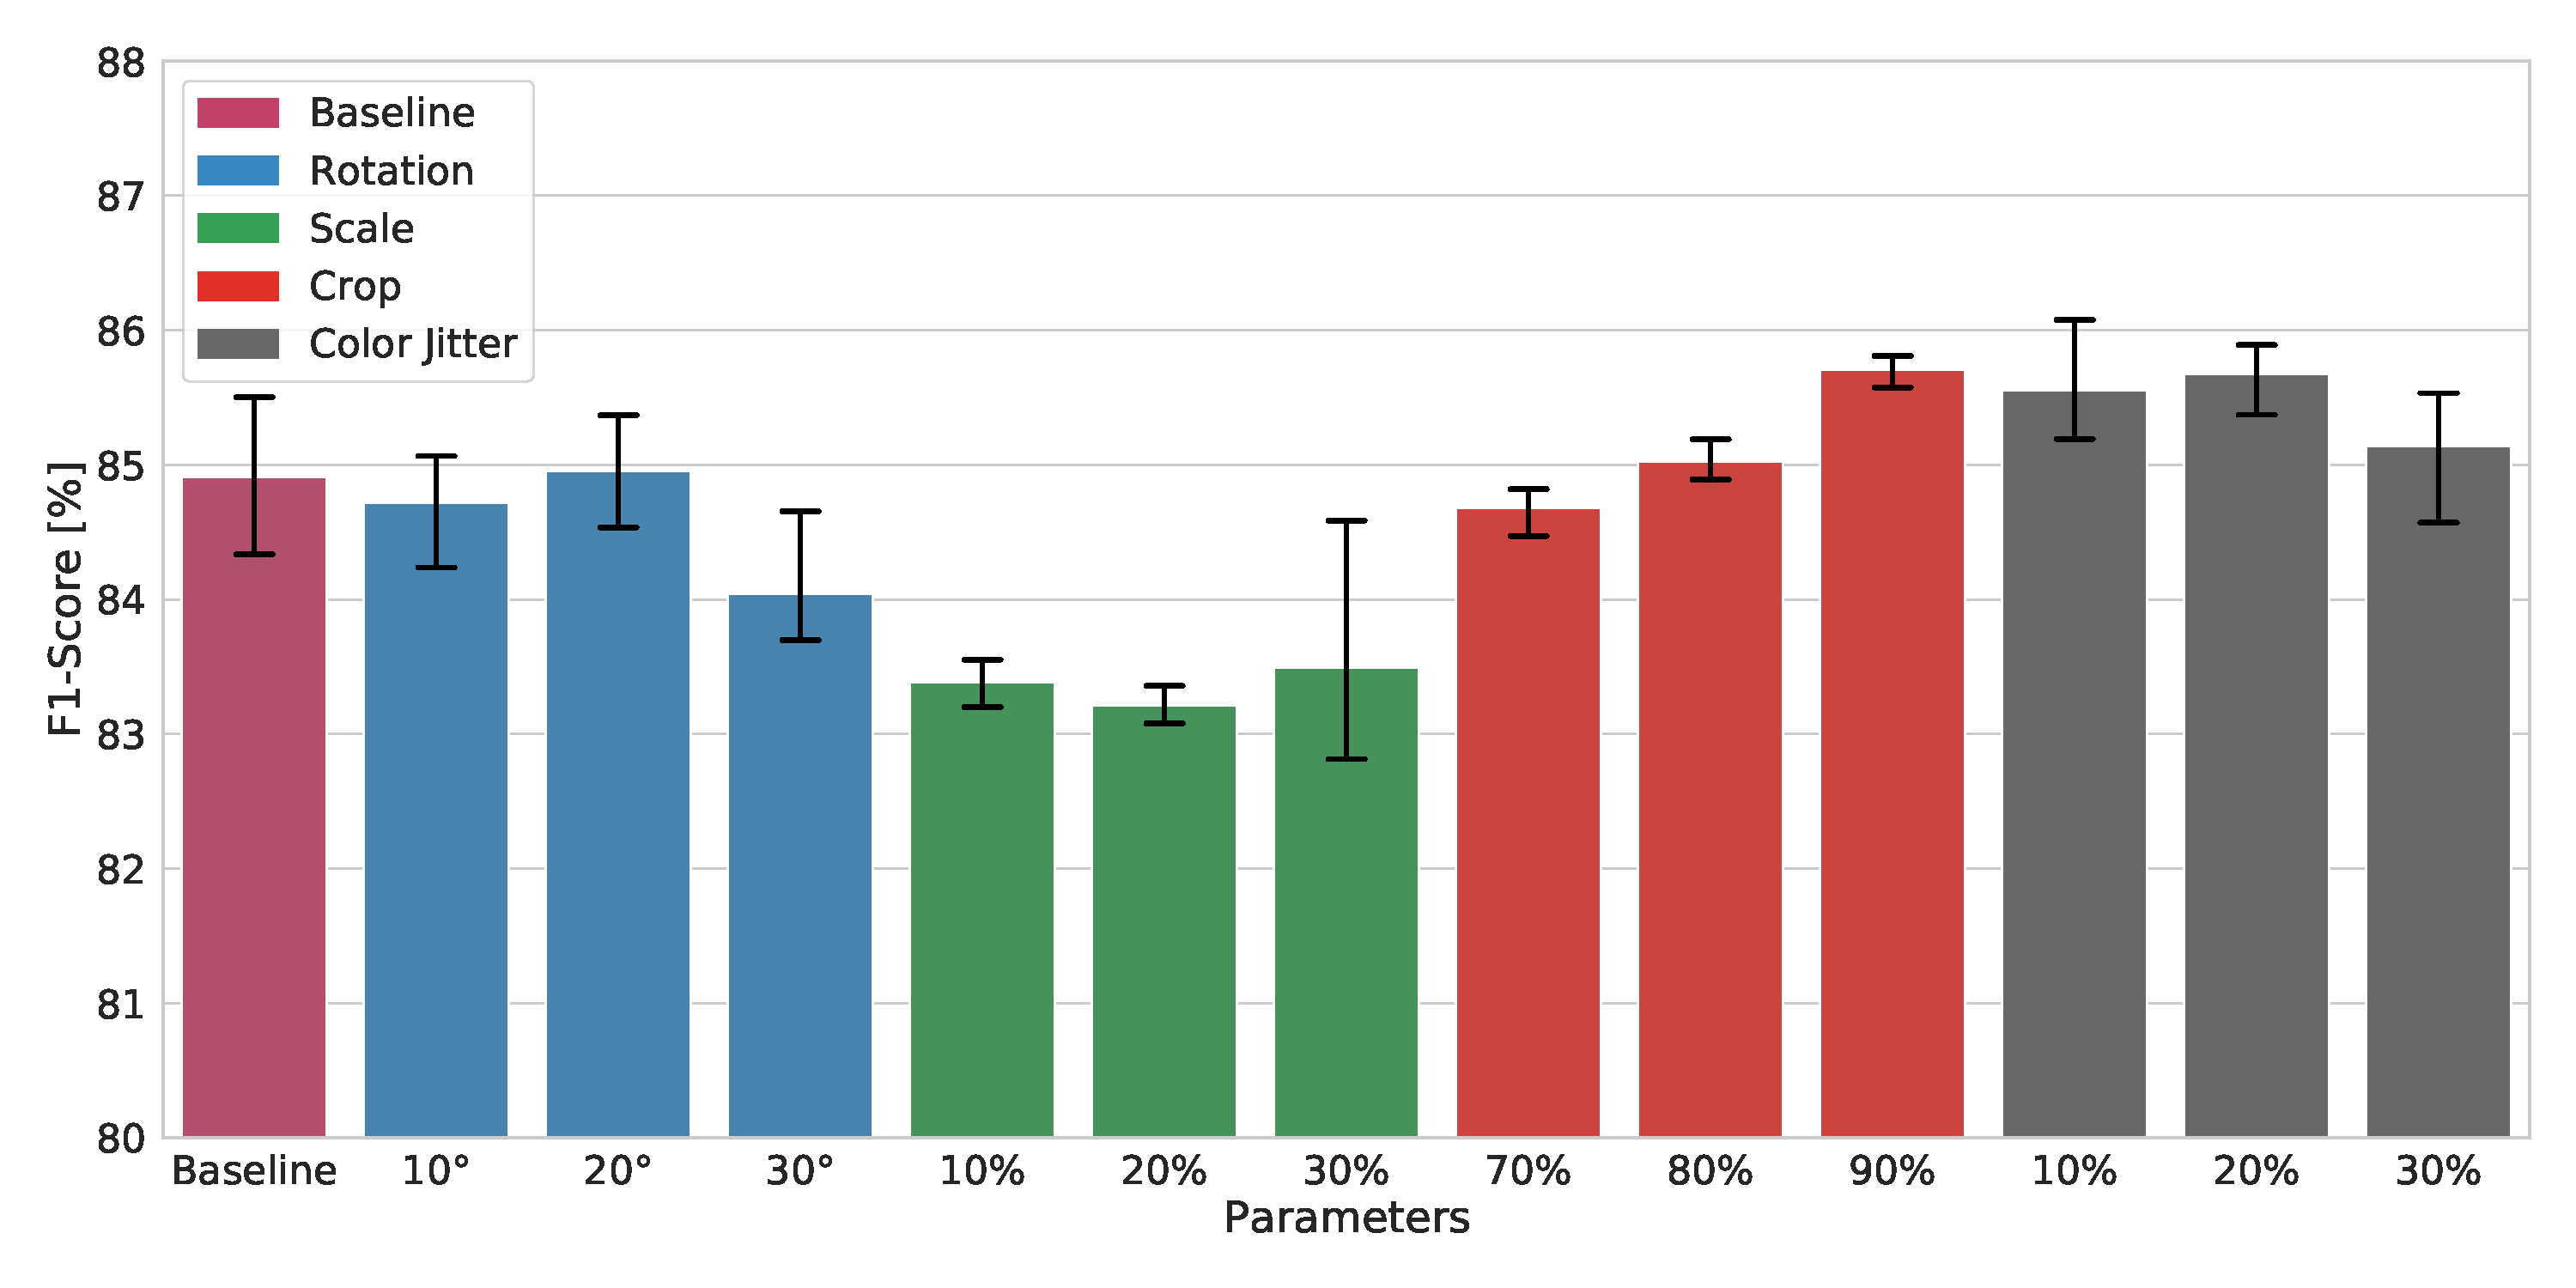
\includegraphics[width=\columnwidth]{imgs/munet_online_aug_experiment.pdf}
    \caption{The results of the online augmentation experiment shown on the validation set, as the mean F1-Score of three separate training runs.}
    \label{fig:munet_online_exp}
\end{center}
\end{figure}

\subsubsection{Experiment: Grid Search}

The final training experiment of the \ac{MUnet} was formed by an extensive grid search to obtain the optimal parameters for the training.
The grid search was performed on the following parameters:

\begin{table}[H]
\footnotesize
\begin{center}
\begin{tabular}{|l|l|}

\hline
\textbf{Learning Rates} & $1.0e^{-2}, 5.0e^{-3}, 2.5e^{-3}, 1.0e^{-3}, 5.0e^{-4}, 2.5e^{-4}, 1.0e^{-4}$ \\
\hline
\textbf{Batch Size} & $32, 64$ \\
\hline
\textbf{Losses} & focal ($\alpha = 0.8, \gamma = 2$), focal ($\alpha = 0.1, \gamma = 2$), dice  \\
\hline
\textbf{Offline Augmentations} & projection, flip, rotation \\
\hline
\textbf{Online Augmentations} & rotation = 20\textdegree, crop = 90\%, color jitter = 20\% \\
\hline

\end{tabular}
\caption{Configuration of the \ac{MUnet} grid search experiment. The networks were trained for all possible combinations of learning rate, batch size and loss function.}
\label{tab:munet_grid_params}
\end{center}
\end{table}

The results of the grid search experiment were first evaluated on the validation set and performance is shown for the three different metrics f1-score, recall and precision.
Further, the evaluation was split up and the three metrics were calculated on the whole validation set and only on the checkered images in the validation set.
This distinction was done to see whether the data is biased towards non-checkered images or not.
The results of the three metrics on the full validation set are shown in the figures \ref{fig:munet_f1b_heat}, \ref{fig:munet_rb_heat} and \ref{fig:munet_pb_heat}, respectively.
The results on only checkered images can be found in the figures \ref{fig:munet_f1c_heat}, \ref{fig:munet_rc_heat} and \ref{fig:munet_pc_heat}, respectively.
In the following a fold is defined as a combination of loss and batch size.

When looking at the f1-score on the full validation set (fig. \ref{fig:munet_f1b_heat}), no clear sign can be observed that a one batch size performs better than another.
Furthermore, all focal loss folds seem to be robust in terms of differing learning rates, however the same does not apply to the dice loss folds, which show with a decreasing learning rate, also a decrease in f1-score.
The decrease in f1-score in the dice loss folds is related to a drop in precision (fig. \ref{fig:munet_pb_heat}), but on the other hand-side an increase in recall (fig. \ref{fig:munet_rb_heat}).
The best performing learning rates can be found for the higher learning rates ranging from $2.5e^{-3}$ to $1.0e^{-2}$.

Inspecting now the f1-score on the validation set for checkered images only (fig. \ref{fig:munet_f1c_heat}), the best learning rates can be found in the middle and low range ($1.0^e{-4}$ - $1.0e^{-3}$), which leads to the assumption that higher learning rates probably perform better on non-checkered images, and lower learning rates perform better on checkered images.
Comparing the different loss configurations based on their batch size shows that a higher batch size seems to perform slightly better on the checkered images.
Furthermore, the dice loss against shows poor performance on small learning rates.

For the final evaluation from each fold six networks are selected.
This networks were chosen based on the best performing metrics, where three networks were chosen based on the best f1-score, precision and recall on the full validation set.
And the other three were selected for the same metrics, based only on the checkered images from the validation set.
If a network was the best performing on more than one metric no other network was selected from that fold, hence the amount of networks was reduced.
The selected folds based on their best performing metric can be found in table \ref{tab:munet_selected_nets}.
Overall there were six folds (three loss functions * two batch sizes), each fold was tested for three metrics on two datasets (f1-score, precision and recall * (full validation set + checkered validation set)), therefore in theory there were a maximum of 36 network candidates.
Some networks were the best on multiple metrics, therefore the actual number of selected networks was 26.

The selected networks were now used for further testing and the performance on the validation and test dataset can be found in the figures \ref{fig:munet_fold_32} and \ref{fig:munet_fold_64}, for the batch size of 32 and 64 respectively.
When looking at both fold types based on the batch size for the focal loss types a decreasing trend in f1-score can be observed on the validation set, however on the test set the f1-score is increasing.
This leads even more to the assumption that the high learning rate, chosen in the initial learning rate search experiment, leads to an overfitting on the validation set and a smaller learning rate would have been more adequate.
Further, again the worst performing networks are those trained with the dice loss and a low learning rate combination, which already showed bad validation and now again showed bad test performance of around 50\% f1-score.
In general the best learning rates can be found in the middle and lower learning rate range.
